%!TEX root = ../thesis.tex

\chapter{Основні відомості про TRNG}
\label{chap:review}  %% відмічайте кожен розділ певною міткою -- на неї наприкінці необхідно посилатись

\section{Що таке TRNG і чому він важливий?}

TRNG (True Random Number Generators) - це функція або пристрій, заснований на непередбачуваному фізичному явищі, що назвиний джерелом ентропії, яке призначене для генерування недетермінованих даних (наприклад, послідовності чисел) для запуску алгоритмів безпеки.

Під'єднані пристрої стають частиною повсякденного життя, і ми очікуємо, що вони працюватимуть коректно, захищаючи ділову та особисту інформацію. PRNG лежать в основі захисту цих пристроїв, оскільки вони використовуються для створення і захисту секретів та іншої конфіденційної інформації. Вони є частиною "ланцюжка довіри", який необхідно створити, починаючи з SoC, переходячи до рівнів додатків і комунікації з хмарою. Ланцюжок довіри сильний лише настільки, наскільки сильна його найслабша ланка.

Непередбачувані генератори випадкових чисел (ГВЧ) відкривають двері для багатьох можливих атак, які можуть зламати пристрої та скомпрометувати дані. Щоб бути ефективними, випадкові числа мають бути непередбачуваними, статистично незалежними (не пов'язаними з раніше згенерованими випадковими числами), рівномірно розподіленими (однакова ймовірність генерації будь-якого числа) і захищеними 


\begin{figure}[h]
  \centering
  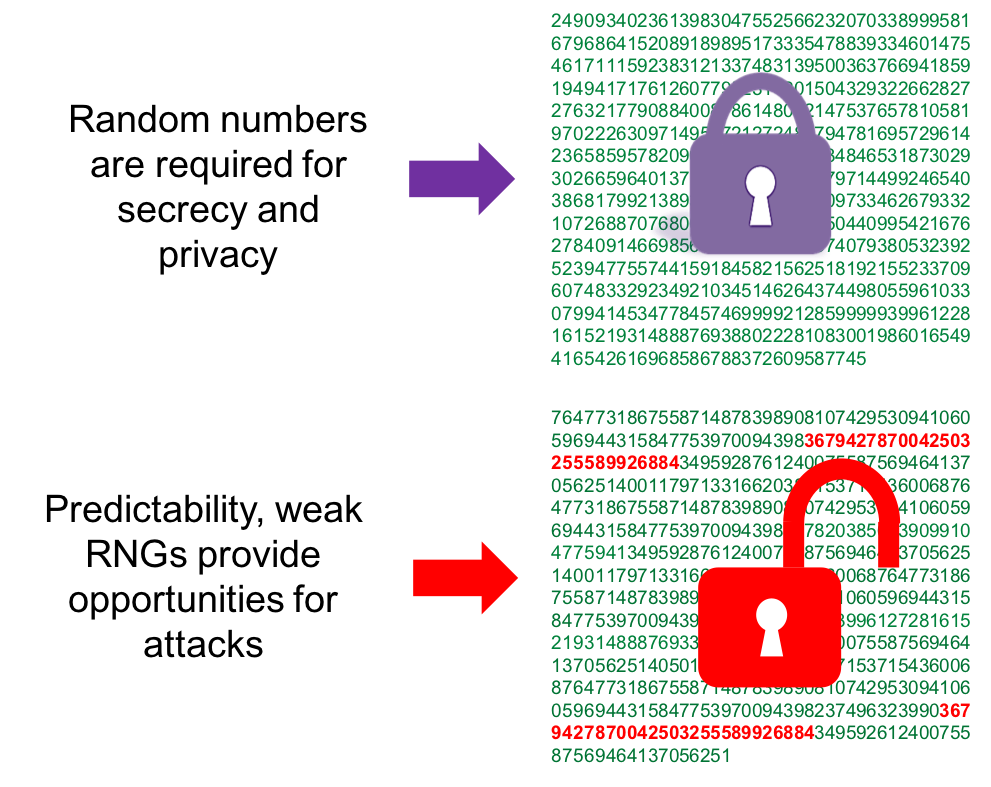
\includegraphics[width=0.8\textwidth]{IMAGES/01.png}
  %\caption{Подпись к картинке}
  \label{fig:fig1}
\end{figure}


\section{Де вони можуть бути використані?}

Справжні випадкові числа використовуються в таких сферах, як азартні ігри та криптографія, де випадковість має вирішальне значення. Наприклад, багато криптографічних алгоритмів і протоколів безпеки залежать від ключів, а їхня міцність визначається кількістю бітів ключа, які необхідно визначити зловмиснику, щоб зламати систему. Якщо ключі скомпрометовані, то під загрозою опиняється безпека всієї системи. 

Справжні випадкові числа потрібні в різних сценаріях безпеки:
\begin{itemize}
  \item Генерація ключів для різних алгоритмів (симетричних, асиметричних, MAC) і протоколів (SSL/TLS, SSH, WiFi, LTE, IPsec тощо).
  \item Виробництво чипів (завдання унікальних ключів пристрою і платформи).
  \item Початкові значення (для алгоритмів шифрування і MAC, значень TCP-пакетів тощо).
  \item Генерація nonce і початкові значення лічильників для різних криптографічних функцій.
  \item Виклики, що використовуються для обміну автентифікацією в протоколі.
  \item Введення рандомізації для рішень з протидії побічним каналам для захисту від фізичних атак.
\end{itemize}


\section{Стандарти для TRNG}

Кілька асоціацій зі стандартизації та сертифікації розробляють специфікації та методи перевірки для TRNG, щоб визначити рекомендації щодо розроблення та сертифікації дійсно випадкових рішень. 

Американський Національний інститут стандартів і технологій (NIST) розробив набір стандартів NIST SP 800-90A/B/c ("c" поки що перебуває на стадії проєкту) для визначення критеріїв статистичного аналізу, яким має задовольняти TRNG, щоб вважатися достатньо випадковим для криптографічних застосувань. Німецький орган зі стандартизації, Bundesamt für Sicherheit in der Informationstechnik (BSI), уже давно має окремий набір стандартів на TRNG (AIS 20/31). 

Обидва стандарти слугують для відсіювання генераторів, що лише здються випадковими, але можуть мати статистичні недоліки, які можуть підірвати безпеку системи. Однак, хоча ці стандарти дають деякі рекомендації щодо архітектури високого рівня, вони не описують конкретно, як створити TRNG; тільки як перевірити, чи працює він. Деталі реалізації залишені на розсуд розробників, що допускає безліч альтернативних підходів. Однак у всіх випадках TRNG повинні відповідати чотирьом критеріям, про які йшлося раніше: вони повинні бути непередбачуваними, одноманітними, незалежними та такими, що їх неможливо виявити.

\begin{figure}[h]
  \centering
  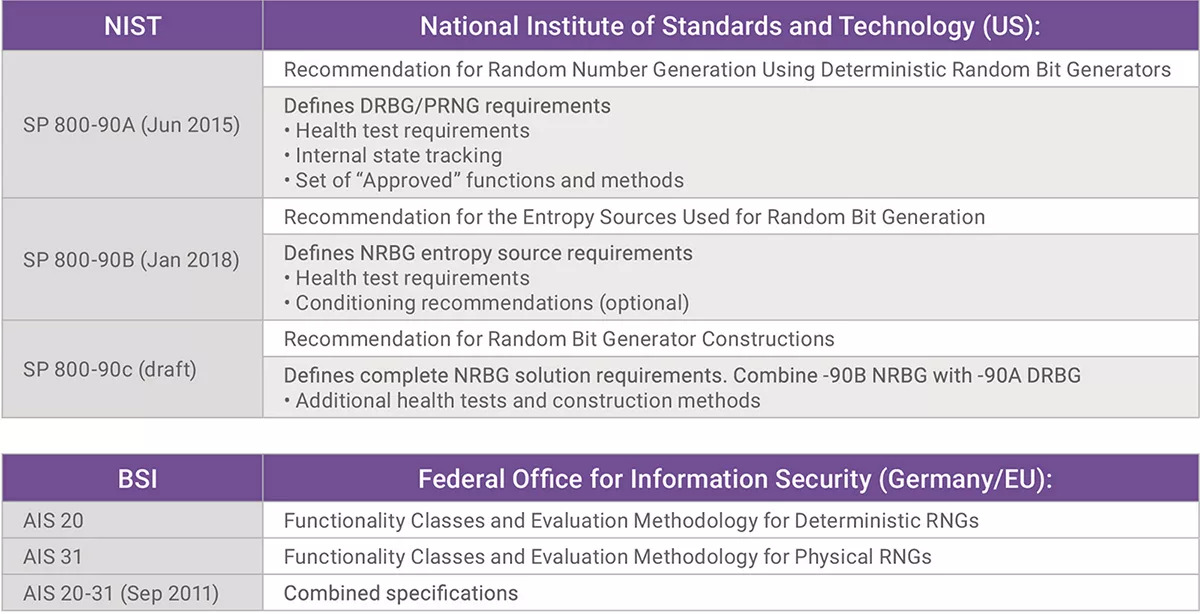
\includegraphics[width=0.8\textwidth]{IMAGES/02.jpg}
  %\caption{Подпись к картинке}
  \label{fig:fig1}
\end{figure}

На додаток до тестів відповідності NIST SP 800-90A/B/c і BIS AIS 20-31, NIST випустив набір статистичних тестів для генераторів випадкових і псевдовипадкових чисел для криптографічних додатків під назвою NIST SP800-20. Однак цих тестів недостатньо для виявлення деяких слабких місць у генераторах випадкових чисел, тому було розроблено інші тести, що доповнюють перевірку рандомізації для TRNG, зокрема набори Diehard і Dieharder. 


Такі сертифікати, як американський федеральний стандарт обробки інформації (FIPS) 140-2 і нещодавно вийшовший 140-3, Common Criteria (CC) і китайський Office of State Commercial Cryptography Administration (OSCCA), покликані забезпечити повну відповідність кінцевих продуктів вимогам, зазначеним у специфікаціях. Спеціалізовані лабораторії перевіряють архітектуру TRNG, оцінюють властивості генерації випадковості, тестують і підтверджують, що продукти дійсно відповідають вимогам.

\section{Рішення TRNG}

Справжньої випадковості домогтися дуже складно. Правильно сконструйований TRNG повинен збирати ентропію з якого-небудь випадкового процесу (наприклад, шуму, створюваного струмом у транзисторі, або часу між подіями радіоактивного розпаду), а потім кондиціонувати ентропійний сигнал, щоб видалити зміщення і вибілити спектр отриманої послідовності виходів. Цей процес потрібно контролювати з урахуванням таких факторів, як робоча температура, старіння, сприйнятливість до електронних шумів і збоїв, зміна напруги та діапазон робочих частот. Без контролю цих чинників схема TRNG може бути модифікована сторонніми особами, які намагаються вплинути на її роботу.

Одним із прикладів архітектури RNG є запуск генератора псевдовипадкових чисел (PRNG) криптографічної якості з невідомим початковим значенням, а потім використання PRNG протягом певного періоду часу або для отримання певної кількості випадкових даних. Потім PRNG буде повторно засіяний і знову використаний протягом деякого часу, і так далі. Як затравку для PRNG слід використовувати секретний випадковий вхідний сигнал, отриманий від "джерела ентропії", такого як високоякісний TRNG.  

\begin{figure}[h]
  \centering
  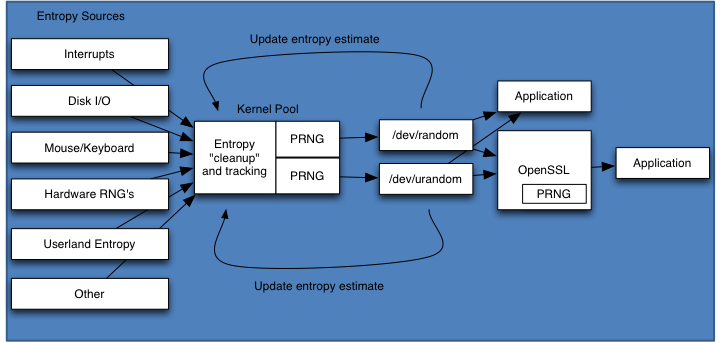
\includegraphics[width=0.8\textwidth]{IMAGES/07.png}
  \label{fig:fig1}
\end{figure}

Як можна бачити, сенс використання PRNG і TRNG разом, можливо, для створення CSPRNG, полягає саме в цьому: після отримання достатньої початкової випадковості, швидкість, рівномірність і ентропія можуть бути досягнуті шляхом безперервного заповнення пулів навіть досить низькоякісними TRNG, а потім вилученням результатів за допомогою ефективного PRNG, наприклад, легкого симетричного шифру або хеш-функції.

Компанія Synopsys, до слова, розробила відповідні стандартам і готові до сертифікації TRNG, які можна застосувати до будь-яких цифрових напівпровідникових пристроїв і які добре переносяться на будь-які ASIC і більшість FPGA-технологій. TRNG широко впроваджуються аж до 5-нм техпроцесів, конфігуруються замовником і підтримують цілу низку привабливих функцій, включно з широким динамічним діапазоном системного тактового генератора, резервуванням та вибором кількості внутрішніх генераторів сідінгу, автоматичним та ручним перезапуском, вихідними потоками для захисту від побічних каналів та різними інтерфейсами (з відображенням у пам'яті, послідовним та nonce, який підходить для модулів захисту контенту HDCP 2.3):

Ядро генератора істинних випадкових чисел DesignWare® належить до класу недетермінованих генераторів випадкових бітів (NRBG). Ядро містить джерело ентропії та схему відбілювання, які генерують рівномірно розподілену випадкову послідовність бітів. Вихідні дані DesignWare TRNG можна використовувати безпосередньо або для засіву/заправлення детермінованого генератора випадкових бітів (DRBG), схваленого NIST SP 800-90A, залежно від сфери застосування. Випадкові дані, що генеруються DesignWare TRNG, мають бути статистично еквівалентними рівномірно розподіленому шуму. Схема містить генератор сідінгу, який створює недетерміноване випадкове значення для запуску TRNG.

Генератор випадкових чисел DesignWare True Random Number Generator Core for NIST SP 800-90c повністю відповідає специфікаціям NIST SPA800-90A/B/c і BSI AIS 20/31. Він генерує випадкові числа, які статистично еквівалентні рівномірно розподіленому потоку даних. Ядро містить схему кондиціонування, схвалену NIST SP800-90B, із сумісним джерелом шуму і DRBG, схвалену NIST SP800-90A. Ядро підтримує високопродуктивні операції (3,2 Гбіт/с за частоти 500 МГц) для генерації випадкових чисел, які мають бути статистично еквівалентними рівномірно розподіленому потоку даних. За кремнієвої реалізації DesignWare TRNG може відповідати найвищим комерційним і державним стандартам і підтримувати сертифікацію кінцевих продуктів, включно з FIPS 140-2 / 140-3, Common Criteria і OSCCA. У ядро можна включити до 8 віртуальних TRNG, що забезпечує можливість безпечного доступу до випадкових чисел між декількома користувачами, наприклад, у багатоядерній процесорній системі. ІС також підтримує збір фонового шуму для генерації нової ентропії у фоновому режимі та збереження її для наступної операції сідінгу, що усуває час очікування наступного засіву.